% Provenance (never printed): see sources/outline_sources.md (Year 3: the heat
% equation, half-space and plate cooling models, heat flow against age,
% continental geotherms, thermal subsidence). Brief: sources/book5/BRIEFS.md,
% ch. 5. Curves from figdata/bachelor-3/plate_cooling.py (models; Seton et al.
% 2020 age grid and ETOPO1, read only) and continental_geotherm.py.
% Exercise and problem values in the Book 5 scratch calculator calc/ch05.py.
\chapter{Modelos térmicos de la litosfera}\label{ch:b3:lithosphere-thermal-models}

Al alejarse de una dorsal oceánica, el fondo marino se hace más profundo: unos
\qty{2.5}{km} en el eje, y más de \qty{5}{km} bajo el fondo oceánico más
antiguo. No se ha añadido nada a la placa ni se le ha quitado nada; solo se ha
enfriado, contraído y hundido. El fondo oceánico es un termómetro de la placa
que tiene debajo, y una sonda de flujo de calor hincada en sus sedimentos registra el mismo
enfriamiento desde arriba. Este capítulo resuelve el enfriamiento de una placa de dos maneras,
como semiespacio y como placa de espesor finito, compara ambas con la profundidad
real del fondo oceánico y con su flujo de calor, y luego se ocupa de los continentes,
cuyo calor procede en parte de su propia corteza.
% ledger: ps77:depth-age

\begin{recall}
La ecuación de difusión del calor, $\partial T/\partial t = \kappa\nabla^2T$,
con la conductividad térmica $k$ y la difusividad térmica $\kappa =
k/(\rho c)$, es de los libros de física; las series de Fourier y la función de error
$\operatorname{erf}x = (2/\sqrt\pi)\int_0^xe^{-u^2}\,\mathrm du$ están en los
volúmenes universitarios de los libros de matemáticas. El flujo de calor, la producción de calor
radiogénico, la geoterma, la escala de tiempo conductivo $L^2/\kappa$, la
capa límite térmica y la litosfera térmica se definieron en el volumen de primer año,
en su capítulo sobre el balance térmico terrestre; la isostasia, en su capítulo sobre
isostasia y anomalías de la gravedad; la ley profundidad--edad $d = d_r + C\sqrt t$ se demostró en
su capítulo sobre rifts, dorsales y márgenes pasivos, al admitir el perfil de temperatura
que este capítulo deriva. El modelo de estiramiento de cuencas, la subsidencia
postrift y la constante de tiempo térmica están en el volumen de segundo año, en su
capítulo sobre cuencas sedimentarias.
\end{recall}

\section{Conducción, advección y su razón}

El calor de la litosfera se mueve de dos maneras: se difunde a favor del gradiente de temperatura,
y lo transporta la roca en movimiento: la placa que abandona una dorsal, una
montaña erosionada que se eleva, un magma que asciende. Cuál de los dos mecanismos prevalece
depende de un único número.

\begin{definition}[Número de Péclet térmico]\label{def:b3:lithosphere-thermal-models:peclet}
Para una roca que se mueve a la velocidad $u$ a lo largo de una longitud $L$, el \emph{número de Péclet
térmico}\index{número de Péclet térmico} es
\[
  \mathrm{Pe} = \frac{uL}{\kappa},
\]
la razón entre el tiempo conductivo $L^2/\kappa$ y el tiempo advectivo $L/u$.
La advección domina donde $\mathrm{Pe} \gg 1$, y la conducción donde
$\mathrm{Pe} \ll 1$.
\end{definition}

Una placa que abandona una dorsal a \qty{25}{mm/yr} tiene, a lo largo de una distancia de
\qty{95}{km}, $\mathrm{Pe} \approx 94$ con $\kappa = \qty{0.8e-6}{m^2.s^{-1}}$:
el calor es arrastrado lateralmente por la placa mucho más deprisa de lo que se difunde lateralmente.
Cada columna vertical de la placa se enfría, por tanto, como si estuviera sola, por conducción vertical
hacia el fondo marino frío, siendo la edad $t$ el tiempo transcurrido desde que
abandonó el eje. Así, un problema en dos dimensiones se convierte en uno de profundidad
y tiempo.

\section{El semiespacio en enfriamiento}

\begin{definition}[Modelo de enfriamiento de semiespacio]\label{def:b3:lithosphere-thermal-models:half-space}
El \emph{modelo de enfriamiento de semiespacio}\index{modelo de enfriamiento de semiespacio} de la
litosfera oceánica toma cada columna como un semiespacio $z \ge 0$ de difusividad uniforme,
a la temperatura uniforme $T_m$ del manto cuando abandona el
eje de la dorsal, cuya superficie se mantiene desde entonces a la temperatura $T_0$ del
fondo marino, sin producción de calor y sin base.
\end{definition}

\begin{theorem}[Geoterma de función de error]\label{thm:b3:lithosphere-thermal-models:erf}
En el \omterm{def:b3:lithosphere-thermal-models:half-space}{modelo de enfriamiento de semiespacio}, la temperatura a la profundidad $z$ bajo el
fondo marino de edad $t$ es
\[
  T(z, t) = T_0 + (T_m - T_0)\operatorname{erf}\frac{z}{2\sqrt{\kappa t}} .
\]
Esta es la \emph{geoterma de función de error}\index{geoterma de función de error}.
\end{theorem}

\begin{proof}
Sea $\theta = (T - T_0)/(T_m - T_0)$; satisface $\partial\theta/\partial t =
\kappa\,\partial^2\theta/\partial z^2$ con $\theta(z, 0) = 1$ para $z > 0$ y
$\theta(0, t) = 0$ para $t > 0$. El problema no tiene escala de longitud propia:
si $\theta(z, t)$ es una solución, también lo es $\theta(\lambda z, \lambda^2t)$ para todo
$\lambda > 0$, con los mismos valores inicial y de contorno; siendo la solución
única, $\theta$ depende de $z$ y $t$ solo a través de $\eta = z/(2\sqrt{\kappa
t})$. Escribiendo $\theta = f(\eta)$, con $\partial\eta/\partial t = -\eta/(2t)$ y
$\partial\eta/\partial z = 1/(2\sqrt{\kappa t})$,
\[
  -\frac{\eta}{2t}f'(\eta) = \kappa\,\frac{f''(\eta)}{4\kappa t},
  \qquad\text{luego}\qquad f'' + 2\eta f' = 0 .
\]
Así, $f' = Ae^{-\eta^2}$ y $f = A\int_0^\eta e^{-u^2}\,\mathrm du + B$. La
condición de superficie, en $\eta = 0$, da $B = 0$; la condición inicial, que
se cumple a cualquier profundidad cuando $t \to 0$, es decir, cuando $\eta \to \infty$, da
$A\sqrt\pi/2 = 1$. Por tanto, $f = \operatorname{erf}\eta$.
\end{proof}

La temperatura a una profundidad dada depende solo de $z/\sqrt t$: una isoterma se hunde
como la raíz cuadrada de la edad, y la capa enfriada a \qty{40}{Myr} tiene el doble
de espesor que a \qty{10}{Myr}. El flujo de calor en superficie se obtiene por derivación.

\begin{proposition}[Relación flujo de calor--edad]\label{prop:b3:lithosphere-thermal-models:heat-flow}
En el \omterm{def:b3:lithosphere-thermal-models:half-space}{modelo de enfriamiento de semiespacio}, el flujo de calor a través del fondo marino de edad $t$
es
\[
  q(t) = k\,\frac{\partial T}{\partial z}\Big|_{z=0}
  = \frac{k(T_m - T_0)}{\sqrt{\pi\kappa t}} = \frac{C_q}{\sqrt t} .
\]
\end{proposition}

\begin{proof}
$\partial\operatorname{erf}(z/2\sqrt{\kappa t})/\partial z = (2/\sqrt\pi)
e^{-z^2/4\kappa t}/(2\sqrt{\kappa t})$, que en $z = 0$ vale $1/\sqrt{\pi\kappa
t}$.
\end{proof}

Con los valores del modelo de placa indicados a continuación ($k = \qty{3.1}{W.m^{-1}.K^{-1}}$,
$T_m - T_0 = \qty{1450}{K}$, $\kappa = \qty{0.8e-6}{m^2.s^{-1}}$), $C_q =
\qty{505}{mW.m^{-2}.Myr^{1/2}}$, cercano a los valores de 430 a
\qty{510}{mW.m^{-2}.Myr^{1/2}} ajustados a las medidas globales de distintos
estudios; una compilación reciente prefiere \num{490}. El flujo de calor medido sobre la
corteza oceánica joven, sin embargo, subestima de forma notable el calor que sale de ella:
el agua de mar que circula por la corteza agrietada se lleva parte del calor
en fuentes hidrotermales, fuera del alcance de las sondas. Sobre la corteza antigua, las mediciones
siguen $1/\sqrt t$, y las estimaciones de la pérdida de calor terrestre sustituyen las
mediciones sobre la corteza más joven que \qty{66.5}{Myr} por $C_q/\sqrt t$.
% ledger: honda04:gdh1, b2dd10:half-space, dd10b5:hydrothermal

El volumen de primer año integró el mismo perfil en profundidad, mediante la isostasia, para
obtener la ley profundidad--edad, $d = d_r + C\sqrt t$ con $C = 2\rho_m\alpha(T_m -
T_0)\sqrt\kappa/\bigl(\sqrt\pi(\rho_m - \rho_w)\bigr)$ (figura de abajo). Con
$\rho_m = \qty{3300}{kg.m^{-3}}$, $\rho_w = \qty{1030}{kg.m^{-3}}$ y $\alpha =
\qty{3.1e-5}{K^{-1}}$, $C = \qty{370}{m.Myr^{-1/2}}$, frente a los
\qty{350}{m.Myr^{-1/2}} ajustados a los fondos del Pacífico Norte y del Atlántico Norte
más jóvenes que \qty{70}{Myr}.
% ledger: ps77:depth-age

\begin{omfigure}
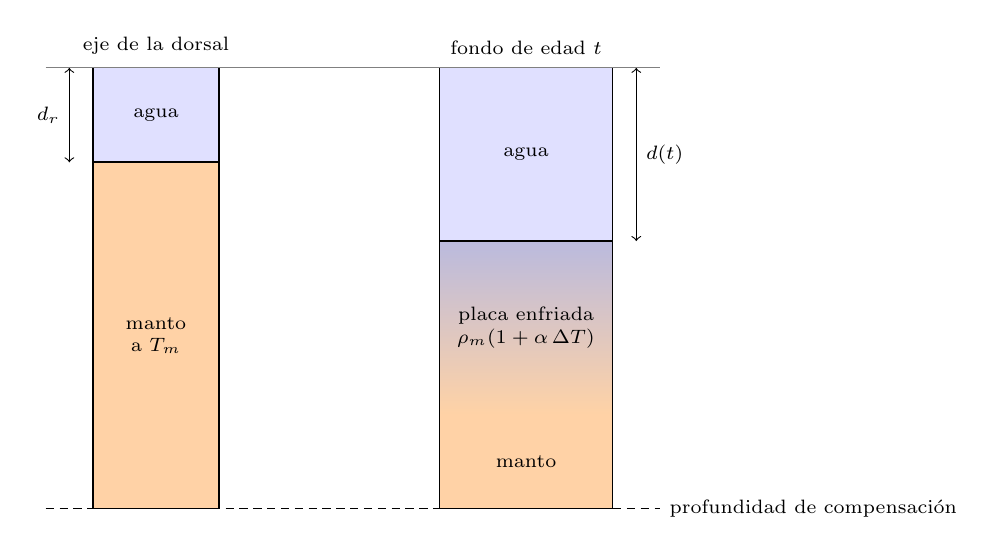
\begin{tikzpicture}[font=\small, x=1cm, y=1cm]
% schematic: two columns of equal mass above the compensation depth
\fill[blue!12] (0,0) rectangle (1.6,-1.2);
\fill[orange!35] (0,-1.2) rectangle (1.6,-5.6);
\fill[blue!12] (4.4,0) rectangle (6.6,-2.2);
\shade[top color=blue!35!gray!40, bottom color=orange!35] (4.4,-2.2) rectangle (6.6,-4.4);
\fill[orange!35] (4.4,-4.4) rectangle (6.6,-5.6);
\draw (0,0) rectangle (1.6,-5.6) (4.4,0) rectangle (6.6,-5.6);
\draw[densely dashed] (-0.6,-5.6) -- (7.2,-5.6) node[right, font=\scriptsize] {profundidad de compensación};
\draw[thick] (0,-1.2) -- (1.6,-1.2) (4.4,-2.2) -- (6.6,-2.2);
\node[font=\scriptsize] at (0.8,-0.6) {agua};
\node[font=\scriptsize, align=center] at (0.8,-3.4) {manto\\a $T_m$};
\node[font=\scriptsize] at (5.5,-1.1) {agua};
\node[font=\scriptsize, align=center] at (5.5,-3.3) {placa enfriada\\$\rho_m(1 + \alpha\,\Delta T)$};
\node[font=\scriptsize, align=center] at (5.5,-5.0) {manto};
\draw[<->] (-0.3,0) -- (-0.3,-1.2) node[midway, left, font=\scriptsize] {$d_r$};
\draw[<->] (6.9,0) -- (6.9,-2.2) node[midway, right, font=\scriptsize] {$d(t)$};
\node[above, font=\scriptsize] at (0.8,0.05) {eje de la dorsal};
\node[above, font=\scriptsize] at (5.5,0.05) {fondo de edad $t$};
\draw[gray] (-0.6,0) -- (7.2,0);
\end{tikzpicture}

\par\smallskip{\small Isostasia de la placa en enfriamiento: la columna en la dorsal
y la columna de edad $t$ tienen la misma masa por encima de la profundidad de compensación. La
placa enfriada y más densa se hunde, y el agua ocupa el espacio sobre
ella.}\label{fig:b3:lithosphere-thermal-models:columns}
\end{omfigure}

\section{El modelo de placa}

El fondo oceánico antiguo deja de profundizarse: en el Pacífico Norte y el Atlántico Norte la
profundidad se aparta de $\sqrt t$ entre 60 y \qty{80}{Myr}, y el flujo de calor
se estabiliza. El semiespacio sigue enfriándose indefinidamente; algo debe mantener caliente la base de la
placa caliente.
% ledger: parsons:plate-model

\begin{definition}[Modelo de enfriamiento de placa]\label{def:b3:lithosphere-thermal-models:plate}
El \emph{modelo de enfriamiento de placa}\index{modelo de enfriamiento de placa} de la
litosfera oceánica toma cada columna como una capa $0 \le z \le L$ de difusividad
uniforme, a una temperatura uniforme $T_m$ al salir de la dorsal, cuya
superficie se mantiene a $T_0$ y cuya base se mantiene a $T_m$ desde entonces.
\end{definition}

\begin{theorem}[Serie de temperatura del modelo de placa]\label{thm:b3:lithosphere-thermal-models:plate-series}
En el \omterm{def:b3:lithosphere-thermal-models:plate}{modelo de enfriamiento de placa}, con $T_0 = 0$,
\[
  T(z, t) = T_m\Bigl[\frac zL + \frac2\pi\sum_{n=1}^\infty\frac1n
  \sin\frac{n\pi z}{L}\,e^{-n^2t/\tau}\Bigr],\qquad
  \tau = \frac{L^2}{\pi^2\kappa} .
\]
Esta es la \emph{serie de temperatura del modelo de placa}\index{serie de temperatura del modelo de placa}.
\end{theorem}

\begin{proof}
El estado estacionario, alcanzado cuando $t \to \infty$, es el perfil lineal $T_mz/L$.
La desviación $u = T - T_mz/L$ satisface la ecuación de difusión con $u = 0$ en
$z = 0$ y $z = L$, y parte de $u(z, 0) = T_m(1 - z/L)$. Separando las
variables, $u = Z(z)\Theta(t)$ conduce a $Z''/Z = \Theta'/(\kappa\Theta) = -\mu^2$;
las condiciones de contorno dejan $Z = \sin(n\pi z/L)$, $\mu = n\pi/L$, y
$\Theta = e^{-n^2\pi^2\kappa t/L^2} = e^{-n^2t/\tau}$. Los valores iniciales fijan los
coeficientes $b_n$ de la serie de senos de $T_m(1 - z/L)$ en $[0, L]$:
\[
  b_n = \frac2L\int_0^LT_m\Bigl(1 - \frac zL\Bigr)\sin\frac{n\pi z}{L}\,\mathrm dz
  = \frac{2T_m}{n\pi},
\]
por integración por partes. Sumando los modos se obtiene la serie.
\end{proof}

Cada modo decae con su propio tiempo, $\tau/n^2$: los armónicos superiores, la
estructura fina del escalón inicial, desaparecen primero, y tras un tiempo del orden de $\tau$
solo queda el primero. La misma separación de variables proporciona el flujo de calor
y, mediante el equilibrio isostático de la figura anterior, la profundidad.

\begin{proposition}[Profundidad y flujo de calor del modelo de placa]\label{prop:b3:lithosphere-thermal-models:plate-depth}
En el \omterm{def:b3:lithosphere-thermal-models:plate}{modelo de enfriamiento de placa}, con las densidades y el coeficiente de expansión de la
ley profundidad--edad,
\[
  q(t) = \frac{kT_m}{L}\Bigl[1 + 2\sum_{n=1}^\infty e^{-n^2t/\tau}\Bigr],\qquad
  d(t) = d_r + \frac{\rho_m\alpha T_mL}{2(\rho_m - \rho_w)}
  \Bigl[1 - \frac{8}{\pi^2}\sum_{n\ \text{impar}}\frac{e^{-n^2t/\tau}}{n^2}\Bigr].
\]
Cuando $t \to \infty$, la profundidad tiende a $d_r + \rho_m\alpha T_mL/\bigl(2(\rho_m -
\rho_w)\bigr)$ y el flujo de calor a $kT_m/L$, ambos de forma exponencial, con la
constante de tiempo $\tau$.
\end{proposition}

\begin{proof}
Derivando la serie en $z = 0$, $\partial T/\partial z = (T_m/L)[1 +
2\sum e^{-n^2t/\tau}]$. Para la profundidad, el equilibrio isostático da $(\rho_m -
\rho_w)(d - d_r) = \rho_m\alpha\int_0^L(T_m - T)\,\mathrm dz$. La parte lineal
aporta $T_mL/2$; cada modo aporta $-(2T_m/n\pi)e^{-n^2t/\tau}
\int_0^L\sin(n\pi z/L)\,\mathrm dz = -(2T_m/n\pi)(L/n\pi)(1 - \cos n\pi)
e^{-n^2t/\tau}$, que es nula para $n$ par y $-(4T_mL/n^2\pi^2)
e^{-n^2t/\tau}$ para $n$ impar. Sacando factor común $T_mL/2$ se obtiene el corchete. En $t = 0$
se anula, ya que $\sum_{n\ \text{impar}}1/n^2 = \pi^2/8$.
\end{proof}

El modelo de placa que mejor ajusta las profundidades y los flujos de calor globales tiene una placa
de \qty{95}{km} de espesor, con la base a \qty{1450}{\celsius}, $\alpha =
\qty{3.1e-5}{K^{-1}}$ y $k = \qty{3.1}{W.m^{-1}.K^{-1}}$, más delgada y más caliente
que la anterior, de \qty{125}{km} y \qty{1350}{\celsius}. Con $\kappa =
\qty{0.8e-6}{m^2.s^{-1}}$, $\tau = \qty{36.2}{Myr}$; la profundidad se estabiliza en
$2500 + 3104 = \qty{5604}{m}$ y el flujo de calor en \qty{47}{mW.m^{-2}}. El fondo
joven no permite distinguir entre los dos modelos: difieren en menos de un metro a
\qty{2}{Myr} y en \qty{100}{m} a \qty{44}{Myr}. La sismología da una respuesta
parecida: las \omterm{def:b3:seismology-imaging:surface-waves}{ondas de Rayleigh} del Pacífico se ajustan mejor a placas en enfriamiento cuyo
espesor asintótico es de 85 a \qty{95}{km}.
% ledger: honda04:gdh1, ps77:depth-age, fischer:lithosphere

\begin{omfigure}
\begin{tikzpicture}
\begin{groupplot}[group style={group size=1 by 2, vertical sep=2.3cm},
  omrecord, width=0.86\linewidth, height=0.42\linewidth, xmin=0, xmax=160,
  xlabel={edad del fondo oceánico (Myr)}]
\nextgroupplot[omdepth, ylabel={profundidad (km)}, ymin=0, ymax=130,
  title={(a) isotermas, cada \qty{200}{\celsius}}, title style={font=\small},
  legend style={font=\scriptsize, at={(0.01,0.03)}, anchor=south west}]
% computed in figdata/bachelor-3/plate_cooling.py; ledger: honda04:gdh1
\addplot[omDef, thick] table[x=t, y=hs200] {figdata/out/bachelor-3-plate_cooling-isotherms.dat};
\addlegendentry{semiespacio}
\addplot[red!70!black, thick, densely dashed] table[x=t, y=pl200] {figdata/out/bachelor-3-plate_cooling-isotherms.dat};
\addlegendentry{placa, $L = \qty{95}{km}$}
\foreach \lev in {400,600,800,1000,1200,1400} {
  \addplot[omDef, thick, forget plot] table[x=t, y=hs\lev] {figdata/out/bachelor-3-plate_cooling-isotherms.dat};
  \addplot[red!70!black, thick, densely dashed, forget plot] table[x=t, y=pl\lev] {figdata/out/bachelor-3-plate_cooling-isotherms.dat};
}
\draw[gray] (axis cs:0,95) -- (axis cs:160,95);
\node[font=\scriptsize, anchor=north] at (axis cs:68,96) {base de la placa};
\node[font=\scriptsize, fill=white, inner sep=1pt] at (axis cs:150,14) {200};
\node[font=\scriptsize, fill=white, inner sep=1pt] at (axis cs:28,38.2) {1000};
\node[font=\scriptsize, fill=white, inner sep=1pt] at (axis cs:22,70.4) {1400};
\nextgroupplot[ylabel={flujo de calor (\unit{mW.m^{-2}})}, ymin=0, ymax=300,
  title={(b) flujo de calor}, title style={font=\small},
  legend style={font=\scriptsize, at={(0.98,0.97)}, anchor=north east}]
\addplot[omDef, thick] table[x=t, y=hs] {figdata/out/bachelor-3-plate_cooling-heat.dat};
\addlegendentry{semiespacio}
\addplot[red!70!black, thick, densely dashed] table[x=t, y=pl] {figdata/out/bachelor-3-plate_cooling-heat.dat};
\addlegendentry{placa}
\end{groupplot}
\end{tikzpicture}

\par\smallskip{\small Los dos modelos de enfriamiento con los parámetros del texto.
(a) Profundidad de las isotermas desde \qty{200}{\celsius} (arriba) hasta
\qty{1400}{\celsius} (abajo): las del semiespacio siguen hundiéndose como
$\sqrt t$, las de la placa se detienen cuando el perfil se vuelve lineal. (b) Flujo de calor
superficial: el modelo de placa se estabiliza en \qty{47}{mW.m^{-2}}; el de semiespacio
decrece como $1/\sqrt t$.}\label{fig:b3:lithosphere-thermal-models:isotherms}
\end{omfigure}

El fondo oceánico real puede representarse en la misma gráfica (figura inferior). Cada celda de
un grado de latitud y longitud cuya edad se conoce se sitúa según su edad y
su profundidad; la mediana de cada intervalo de cinco millones de años aumenta con la edad como predicen los modelos
para los primeros \qty{40}{Myr}, pero el fondo observado es menos profundo que ambos
modelos, y cada vez más con la edad. No se ha corregido nada: el fondo antiguo
tiene una capa de sedimento más gruesa, de más de un kilómetro en el
Atlántico Norte más antiguo, que lo carga y eleva su parte superior, y el fondo antiguo ha tenido tiempo de
acumular montes submarinos, mesetas volcánicas y los abombamientos de los puntos calientes. Los ajustes publicados
eliminan primero la carga de sedimentos y los abombamientos evidentes; la ley profundidad--edad
del volumen de primer año, y los modelos de placa anteriores, proceden de profundidades así
corregidas.
% ledger: data:b5-depth-age, ps77:depth-age

\begin{omfigure}
\begin{tikzpicture}
\begin{axis}[omrecord, omdepth, width=0.86\linewidth, height=0.5\linewidth,
  xmin=0, xmax=180, ymin=2, ymax=6.5, xlabel={edad del fondo oceánico (Myr)},
  ylabel={profundidad (km)},
  legend style={font=\scriptsize, at={(0.5,-0.24)}, anchor=north, cells={anchor=west}},
  legend columns=2]
% computed in figdata/bachelor-3/plate_cooling.py; ledger: data:b5-depth-age, honda04:gdh1
\addplot[only marks, mark=*, mark size=1.3pt, black,
  error bars/.cd, y dir=both, y explicit]
  table[x=t, y expr=\thisrow{med}/1000, y error plus expr=(\thisrow{q3}-\thisrow{med})/1000,
  y error minus expr=(\thisrow{med}-\thisrow{q1})/1000] {figdata/out/bachelor-3-plate_cooling-bins.dat};
\addlegendentry{observada, mediana y cuartiles}
\addplot[omDef, thick] table[x=t, y expr=\thisrow{hs}/1000] {figdata/out/bachelor-3-plate_cooling-depth.dat};
\addlegendentry{semiespacio}
\addplot[red!70!black, thick, densely dashed] table[x=t, y expr=\thisrow{pl}/1000] {figdata/out/bachelor-3-plate_cooling-depth.dat};
\addlegendentry{placa, $L = \qty{95}{km}$}
\end{axis}
\end{tikzpicture}

\par\smallskip{\small Profundidad del fondo oceánico frente a su edad: la mediana y
los cuartiles de las profundidades de las celdas de un grado de cada
intervalo de cinco millones de años (fondo marino más profundo que \qty{1000}{m}, edades de una malla global de edades, profundidades
de un modelo global de relieve, sin corrección por sedimentos, montes submarinos ni abombamientos),
con los dos modelos de enfriamiento del texto.}\label{fig:b3:lithosphere-thermal-models:depth-age}
\end{omfigure}

\begin{definition}[Subsidencia térmica]\label{def:b3:lithosphere-thermal-models:thermal-subsidence}
La \emph{subsidencia térmica}\index{subsidencia térmica} es el hundimiento de la
superficie de la litosfera a medida que se enfría y se contrae hacia el
equilibrio térmico, y el espacio situado encima se llena de agua o sedimento;
la isostasia convierte el calor perdido por una columna en su hundimiento.
\end{definition}

El fondo oceánico es el caso puro. Una cuenca continental estirada es otra: una
litosfera adelgazada por un factor $\beta$ eleva la astenosfera caliente, y la
subsidencia post-rift del volumen de segundo año es el mismo enfriamiento de placa, que parte
de un perfil distinto, con los mismos modos y los mismos tiempos de decaimiento $\tau/n^2$.
Conservar solo el primer modo es, por tanto, una buena aproximación una vez que los superiores
se han extinguido, y una mala antes: para el fondo oceánico del modelo de placa
descrito antes, el primer término por sí solo da la profundidad con un margen de dos metros tras
\qty{20}{Myr}, pero es \qty{84}{m} demasiado profundo a \qty{5}{Myr}.

\section{Geotermas continentales}

La corteza continental produce calor: el granito contiene uranio, torio y potasio en
concentraciones tales que el calor producido en la corteza superior constituye una parte importante del
flujo de calor en la superficie. La forma en que se distribuye la producción con la profundidad
determina la temperatura en profundidad.

\begin{definition}[Escala de profundidad de la producción de calor; flujo de calor reducido]\label{def:b3:lithosphere-thermal-models:reduced}
Cuando la producción de calor radiogénico de la corteza disminuye con la profundidad según
$A(z) = A_0e^{-z/h_r}$, $h_r$ es la \emph{escala de profundidad de la
producción de calor}\index{escala de profundidad de la producción de calor}. El \emph{flujo de
calor reducido}\index{flujo de calor reducido} $q_m$ de una provincia es el flujo de calor que
quedaría en su superficie si la corteza no produjera calor: el flujo de calor procedente de
debajo de la capa radiogénica.
\end{definition}

\begin{proposition}[Producción de calor exponencial]\label{prop:b3:lithosphere-thermal-models:exponential}
En conducción estacionaria con conductividad uniforme $k$, temperatura en la superficie $0$,
producción de calor $A_0e^{-z/h_r}$ y flujo de calor $q_m$ desde gran profundidad, el
flujo de calor superficial es
\[
  q_0 = q_m + A_0h_r,
\]
y la geoterma es
\[
  T(z) = \frac{q_mz}{k} + \frac{A_0h_r^2}{k}\bigl(1 - e^{-z/h_r}\bigr).
\]
Si los plutones de una provincia comparten el mismo $h_r$ y el mismo $q_m$, sus
flujos de calor superficiales y producciones de calor superficiales se sitúan sobre la recta
$q_0 = q_m + h_rA_0$.
\end{proposition}

\begin{proof}
En estado estacionario el flujo de calor ascendente $q(z) = k\,\mathrm dT/\mathrm dz$ disminuye
hacia arriba en la cantidad de calor producido: $\mathrm dq/\mathrm dz = -A(z)$. Con $q \to q_m$
en profundidad, $q(z) = q_m + A_0h_re^{-z/h_r}$, luego $q_0 = q_m + A_0h_r$. Integrando
$\mathrm dT/\mathrm dz = q(z)/k$ desde $T(0) = 0$ se obtiene la geoterma. La última
afirmación es la primera, leída para cada plutón.
\end{proof}

La recta se observa: en varias provincias, los flujos de calor y las producciones de calor superficiales
de los plutones se disponen sobre rectas, con escalas de profundidad de 7.5 a
\qty{10}{km} y un \omterm{def:b3:lithosphere-thermal-models:reduced}{flujo de calor reducido} de \qty{0.8}{HFU} (unos
\qty{33.5}{mW.m^{-2}}) al este de las Montañas Rocosas. La forma exponencial no es
la única que da una recta, pero conserva la recta frente a la erosión: quitar una capa de espesor $e$ desde arriba multiplica
$A_0$ y la parte radiogénica de $q_0$ por el mismo factor $e^{-e/h_r}$.
% ledger: b2roy:provinces

La figura siguiente muestra geotermas para flujos de calor superficiales de 40, 60 y
\qty{80}{mW.m^{-2}}, el primero típico de cratones y el último de zonas de
retroarco, con $k = \qty{2.5}{W.m^{-1}.K^{-1}}$, $h_r = \qty{10}{km}$ y una
aportación cortical $A_0h_r = 0.4\,q_0$. La isoterma de \qty{1300}{\celsius}, tomada como
base de la litosfera térmica, se sitúa a 129, 84 y \qty{61}{km}.
La sismología encuentra manto cratónico rápido hasta unos \qty{250}{km}, y litosfera de retroarco
de 50 a \qty{60}{km} de espesor: las raíces frías y gruesas de los cratones requieren un
\omterm{def:b3:lithosphere-thermal-models:reduced}{flujo de calor reducido} menor del que les asigna este modelo sencillo, y su
conductividad varía con la temperatura, pero el orden de magnitud del contraste es correcto.
% ledger: hyndman:backarc, fischer:lithosphere, delaney86:properties

\begin{omfigure}
\begin{tikzpicture}
\begin{axis}[omrecord, omdepth, width=0.62\linewidth, height=0.6\linewidth,
  xmin=0, xmax=1600, ymin=0, ymax=200, xlabel={temperatura (\unit{\celsius})},
  ylabel={profundidad (km)},
  legend style={font=\scriptsize, at={(0.02,0.03)}, anchor=south west, cells={anchor=west}}]
% computed in figdata/bachelor-3/continental_geotherm.py
\addplot[black, thick] table[x=T40, y=z] {figdata/out/bachelor-3-continental_geotherm-geotherms.dat};
\addlegendentry{$q_0 = \qty{40}{mW.m^{-2}}$}
\addplot[omDef, thick, densely dashed] table[x=T60, y=z] {figdata/out/bachelor-3-continental_geotherm-geotherms.dat};
\addlegendentry{$q_0 = \qty{60}{mW.m^{-2}}$}
\addplot[red!70!black, thick, dashdotted] table[x=T80, y=z] {figdata/out/bachelor-3-continental_geotherm-geotherms.dat};
\addlegendentry{$q_0 = \qty{80}{mW.m^{-2}}$}
\draw[gray, densely dotted] (axis cs:1300,0) -- (axis cs:1300,200);
\node[font=\scriptsize, rotate=90, anchor=south] at (axis cs:1300,160) {\qty{1300}{\celsius}};
\end{axis}
\end{tikzpicture}

\par\smallskip{\small Geotermas continentales estacionarias con
producción de calor decreciente exponencialmente ($h_r = \qty{10}{km}$, $A_0h_r = 0.4\,q_0$, $k =
\qty{2.5}{W.m^{-1}.K^{-1}}$) para tres flujos de calor superficiales. La curvatura cerca de
la superficie se debe al calor propio de la corteza; por debajo de unas pocas escalas de profundidad cada geoterma es
una recta de gradiente $q_m/k$.}\label{fig:b3:lithosphere-thermal-models:geotherms}
\end{omfigure}

\begin{inthefield}[Medición del flujo de calor en el mar]
\begin{minipage}[t]{0.55\linewidth}\vspace{0pt}
Una sonda marina de flujo de calor es una lanza de acero larga con un peso pesado en la parte superior y
un tubo delgado de sensores de temperatura a lo largo de un costado. Desde la popa de un
buque oceanográfico se baja con el cable del torno hasta el fondo marino y se deja caer
en el sedimento blando, con sensores y todo. Permanece inmóvil durante algunos minutos
mientras se disipa el calor por fricción de la penetración y los sensores se estabilizan
a la temperatura del lodo que los rodea: sus lecturas, separadas unos metros, dan
el gradiente de temperatura. Se envía después un pulso breve de calor a lo largo del tubo,
y la velocidad con que se disipa proporciona la conductividad del sedimento que lo rodea;
el producto de ambas magnitudes es el flujo de calor. La lanza se extrae y se vuelve a colocar
unos cientos de metros más adelante a lo largo de la línea, sin volver a
cubierta.
\end{minipage}\hfill
\begin{minipage}[t]{0.42\linewidth}\vspace{0pt}
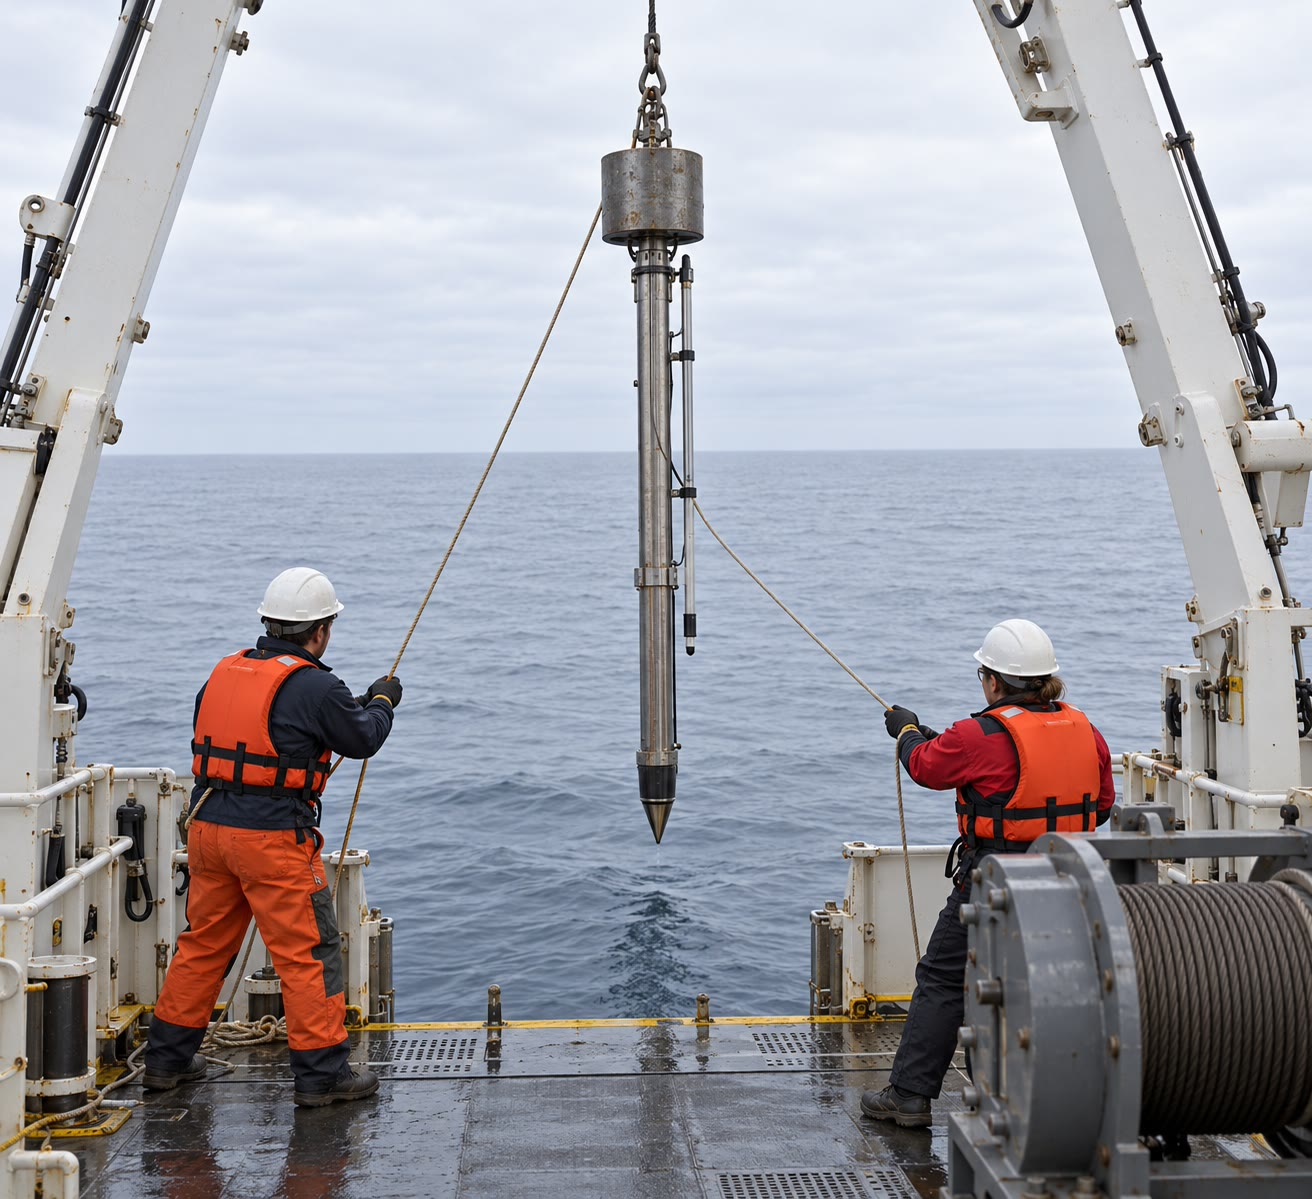
\includegraphics[width=\linewidth]{images/book5/ai/b3-heatflow-probe.jpg}

{\scriptsize Una lanza de medición de flujo de calor a punto de ser arriada desde la popa de un
buque de investigación (Ilustración generada por IA.)}
\end{minipage}
\end{inthefield}

\section{Ejercicios}

\begin{exercise}[$\star$]\label{exo:b3:lithosphere-thermal-models:1}
Con $\kappa = \qty{e-6}{m^2.s^{-1}}$, calcúlese el tiempo conductivo $L^2/\kappa$
para $L = 1$, 10 y \qty{100}{km}, en millones de años.
\end{exercise}

\begin{exercise}[$\star$]\label{exo:b3:lithosphere-thermal-models:2}
Una cordillera se erosiona a razón de \qty{1}{mm/yr}, y la roca asciende a través de los
\qty{30}{km} superiores de corteza para reemplazarla. Con $\kappa = \qty{e-6}{m^2.s^{-1}}$,
calcúlese el número de Péclet. ¿Puede calcularse la geoterma de la cordillera solo
por conducción?
\end{exercise}

\begin{exercise}[$\star$]\label{exo:b3:lithosphere-thermal-models:3}
En el modelo de semiespacio ($T_0 = 0$, $T_m = \qty{1450}{\celsius}$, $\kappa =
\qty{0.8e-6}{m^2.s^{-1}}$), calcúlese la temperatura a \qty{10}{km} bajo el fondo
marino de \qty{5}{Myr} de edad (\qty{1}{Myr} $= \qty{3.156e13}{s}$; $\operatorname{erf}
0.445 = 0.471$).
\end{exercise}

\begin{exercise}[$\star$]\label{exo:b3:lithosphere-thermal-models:4}
Con $C_q = \qty{490}{mW.m^{-2}.Myr^{1/2}}$, calcúlese el flujo de calor a través del
fondo marino de 1, 25 y \qty{100}{Myr} de edad. ¿Cuál de las tres edades subestimaría
con mayor probabilidad una sonda?
\end{exercise}

\begin{exercise}[$\star\star$]\label{exo:b3:lithosphere-thermal-models:5}
En el modelo de semiespacio, la temperatura alcanza el \qty{90}{\percent} de $T_m$
donde $\operatorname{erf}\eta = 0.9$, $\eta = 1.163$. Con $\kappa =
\qty{0.8e-6}{m^2.s^{-1}}$, calcúlese esa profundidad a 10, 40 y \qty{100}{Myr}.
\end{exercise}

\begin{exercise}[$\star\star$]\label{exo:b3:lithosphere-thermal-models:6}
Con los valores del texto, el modelo de semiespacio da $C =
\qty{370.5}{m.Myr^{-1/2}}$. Manteniendo el resto de valores, ¿qué coeficiente de dilatación térmica
daría el valor ajustado \qty{350}{m.Myr^{-1/2}}? ¿Qué otro parámetro
podría modificarse en su lugar?
\end{exercise}

\begin{exercise}[$\star\star$]\label{exo:b3:lithosphere-thermal-models:7}
Calcúlese el flujo de calor asintótico $kT_m/L$ del modelo de placa para $L =
\qty{95}{km}$, $T_m = \qty{1450}{\celsius}$, y para $L = \qty{125}{km}$,
$T_m = \qty{1350}{\celsius}$, con $k = \qty{3.1}{W.m^{-1}.K^{-1}}$ en ambos casos.
¿Cuál se aproxima más al flujo de calor del fondo oceánico antiguo calculado a partir de $C_q/\sqrt t$
a \qty{150}{Myr} con $C_q = \qty{490}{mW.m^{-2}.Myr^{1/2}}$?
\end{exercise}

\begin{exercise}[$\star\star$]\label{exo:b3:lithosphere-thermal-models:8}
Una provincia tiene $q_0 = \qty{60}{mW.m^{-2}}$, $h_r = \qty{10}{km}$ y $A_0h_r =
0.4\,q_0$. Calcúlense $A_0$, $q_m$ y la temperatura en el Moho, a \qty{35}{km}
de profundidad, con $k = \qty{2.5}{W.m^{-1}.K^{-1}}$.
\end{exercise}

\begin{exercise}[$\star\star$]\label{exo:b3:lithosphere-thermal-models:9}
Dos plutones graníticos de una misma provincia dan $q_0 = \qty{66}{mW.m^{-2}}$ con $A_0
= \qty{3.0}{\micro W.m^{-3}}$, y $q_0 = \qty{48}{mW.m^{-2}}$ con $A_0 =
\qty{1.2}{\micro W.m^{-3}}$. Suponiendo que están sobre la recta
de la \cref{prop:b3:lithosphere-thermal-models:exponential}, calcúlense $h_r$ y $q_m$.
\end{exercise}

\begin{exercise}[$\star\star\star$]\label{exo:b3:lithosphere-thermal-models:10}
(a) Demuéstrese que el calor perdido a través del fondo marino entre las edades 0 y $t$, por
unidad de área, es $Q(t) = 2k(T_m - T_0)\sqrt{t/(\pi\kappa)}$ en el modelo de
semiespacio. (b) Demuéstrese que la subsidencia es $d - d_r = \alpha Q/\bigl(c(\rho_m -
\rho_w)\bigr)$, donde $c = k/(\rho_m\kappa)$ es el calor específico. (c) Compruébese
numéricamente a \qty{40}{Myr} con los valores del texto.
\end{exercise}

\begin{exercise}[$\star\star\star$]\label{exo:b3:lithosphere-thermal-models:11}
En el modelo de placa del texto ($\tau = \qty{36.2}{Myr}$, $\rho_m\alpha T_mL/
\bigl(2(\rho_m - \rho_w)\bigr) = \qty{3104}{m}$), la profundidad calculada con el
primer término de Fourier por sí solo supera a la serie completa sobre todo por el término $n = 3$.
Calcúlese el tamaño de ese término a 1, 10 y \qty{20}{Myr}, y la edad a partir de la cual
el primer término por sí solo queda a menos de \qty{10}{m} de la serie.
\end{exercise}

\begin{exercise}[$\star\star\star$]\label{exo:b3:lithosphere-thermal-models:12}
(a) Demuéstrese que, en la geoterma de la \cref{prop:b3:lithosphere-thermal-models:exponential},
$T(z) \approx q_mz/k + A_0h_r^2/k$ para $z \gg h_r$. (b) Dedúzcase la profundidad de la
isoterma de \qty{1300}{\celsius} para $q_0 = \qty{40}{mW.m^{-2}}$, con los valores
del ejercicio 8. (c) ¿En cuánto debe disminuir $q_m$ para que esa profundidad alcance
\qty{250}{km}, la profundidad de las raíces rápidas de los cratones?
\end{exercise}

\section{Problema: cuarenta millones de años lejos de la dorsal}

\begin{problem}[{Problema de fin de semana --- el semiespacio y la placa, la profundidad de
un océano inventado, y el espesor de su placa}]
\label{pb:b3:lithosphere-thermal-models:1}
% values: calc/ch05.py; plate_cooling.py; honda04:gdh1, ps77:depth-age, data:b5-depth-age
Tómense $T_0 = 0$, $T_m = \qty{1450}{\celsius}$, $\kappa =
\qty{0.8e-6}{m^2.s^{-1}}$, $k = \qty{3.1}{W.m^{-1}.K^{-1}}$, $\alpha =
\qty{3.1e-5}{K^{-1}}$, $\rho_m = \qty{3300}{kg.m^{-3}}$, $\rho_w =
\qty{1030}{kg.m^{-3}}$, una dorsal de \qty{2500}{m} de profundidad, y \qty{1}{Myr} $=
\qty{3.156e13}{s}$.

\medskip\noindent\textbf{Parte I --- El semiespacio.}
\begin{enumerate}
  \item Calcúlese $\sqrt{\kappa t}$ a 10 y \qty{40}{Myr}.
  \item Calcúlese la temperatura a \qty{20}{km} bajo el fondo a ambas edades
        ($\operatorname{erf}0.6294 = 0.6266$, $\operatorname{erf}0.3147 =
        0.3437$).
  \item La isoterma de \qty{1000}{\celsius} se sitúa donde $\operatorname{erf}\eta =
        0.6897$, $\eta = 0.7174$. Calcúlese su profundidad a ambas edades, y la edad
        a la que alcanza \qty{60}{km}.
  \item Calcúlese el flujo de calor a ambas edades, y $C_q$.
  \item Una dorsal se abre a \qty{25}{mm/yr} a cada lado. Calcúlese el número de Péclet
        de la placa sobre \qty{95}{km}. ¿Por qué puede enfriarse cada columna
        por separado?
  \item Calcúlese el tiempo conductivo a través de \qty{95}{km}. ¿Qué dice de
        un modelo de semiespacio para un fondo de \qty{150}{Myr} de edad?
\end{enumerate}

\medskip\noindent\textbf{Parte II --- Subsidencia.}
\begin{enumerate}[resume]
  \item Recuérdese el equilibrio isostático que convierte el déficit de temperatura de una
        columna en subsidencia, y por qué la integral puede extenderse hasta el infinito
        en el semiespacio.
  \item Calcúlese $C$ de la ley profundidad--edad, y las profundidades a 10 y
        \qty{40}{Myr}.
  \item La profundidad mediana del fondo oceánico real entre 40 y \qty{45}{Myr}
        es de \qty{4475}{m}, sin corregir. Compárese con el modelo a
        \qty{42.5}{Myr}, y enumérese lo que incluye la mediana y que el modelo
        omite.
  \item ¿En cuánto cambiaría $C$ si $T_m$ fuera \qty{1350}{\celsius}?
        Compárese con el valor ajustado de \qty{350}{m.Myr^{-1/2}}.
  \item ¿Por qué los flujos de calor medidos en fondo joven caen por debajo de $C_q/\sqrt t$?
\end{enumerate}

\medskip\noindent\textbf{Parte III --- La placa.} Tómese $L = \qty{95}{km}$.
\begin{enumerate}[resume]
  \item Calcúlense $\tau$ y la amplitud $\rho_m\alpha T_mL/\bigl(2(\rho_m -
        \rho_w)\bigr)$.
  \item Calcúlese la profundidad a \qty{40}{Myr} con los términos $n = 1$, 3 y 5.
  \item ¿En cuánto difiere el primer término por sí solo de ese valor, y por qué tan
        poco?
  \item Calcúlese la diferencia entre el semiespacio y la placa a 40 y
        \qty{50}{Myr}, y estímese por interpolación lineal la edad a la que
        alcanza \qty{100}{m}.
  \item Calcúlese el flujo de calor de la placa a \qty{40}{Myr}, con los términos
        $n = 1$ a 3, y compárese con el semiespacio.
  \item Dénse la profundidad y el flujo de calor asintóticos.
\end{enumerate}

\medskip\noindent\textbf{Parte IV --- Un océano inventado.} En un océano inventado
cuya dorsal está a \qty{2500}{m} de profundidad, el fondo, una vez corregido por sedimento
y alejado de montes submarinos y elevaciones, está a \qty{5700}{m} de profundidad a \qty{120}{Myr} y
a \qty{4800}{m} a \qty{40}{Myr}. El $L$ de la placa es desconocido; todos los demás valores
son como los anteriores.
\begin{enumerate}[resume]
  \item Conservando solo el primer término de Fourier, escríbase la profundidad a
        \qty{120}{Myr} como función de $L$, con $\tau$ dependiendo a su vez de
        $L$.
  \item Resuélvase para $L$ por iteración, partiendo de $L = \qty{100}{km}$:
        calcúlese $\tau$, después el $L$ que iguala \qty{5700}{m} con ese
        $\tau$, y repítase.
  \item Con el $L$ hallado, calcúlese la profundidad a \qty{40}{Myr} y compárese
        con el semiespacio y con los \qty{4800}{m} medidos.
  \item Calcúlese $\tau$ para ese $L$ y la profundidad asintótica de este océano.
  \item ¿A qué edad el fondo se encuentra a menos de \qty{100}{m} de su
        profundidad asintótica?
  \item Dése el espesor $L$ de la placa que se ajusta al fondo antiguo del
        océano inventado.
\end{enumerate}
\end{problem}
